\chapter{Preliminaries}
\label{sec:prelim}

In this chapter,
we will introduce several key technologies used in our system,
including
DOM tree representation,
Conditional Random Field (CRF) \cite{CRFLafferty},
Stanford Parser\cite{StanfordParser},
Probase\cite{WuLWZ12:Probase},
and short text conceptualization\cite{Song11:Conceptualize}.

These introductions mainly serve as preliminary knowledge so that you can have a better idea
when we discuss the details of our system.
If you are already familiar with these techniques, you can skip this chapter.

\section{DOM Tree Representation}
\label{sec:DOMtree}
In this paper, we focus on the list data of web pages, which are mostly written in HTML.
The Document Object Model, or DOM, presents an HTML page as a tree-structure, which is called DOM tree.
This representation defines a standard way for accessing and manipulating HTML documents
and is widely used in web information extraction and analysis.

\begin{figure}[th]
        \centering
        \epsfig{file=./pics/DOMTree.eps,width=0.9\columnwidth}
        \caption{A HTML sample page(a) and its corresponding DOM tree(b)}
        \label{fig:DOMTree}
\end{figure}

Figure \ref{fig:DOMTree} shows a HTML fragment(a) as well as its corresponding DOM tree(b).
As we can see in the figure, the nodes in the DOM tree have a hierarchical relationship to each other.
Thus we follow the terms used in normal tree structure to describe the DOM tree, such as parent, child, root and leaf.
In an HTML document, there are mainly three kinds of DOM tree nodes.

\begin{itemize}
  \item \textit{Tag node}:
    A tag node represents an HTML element, such as a title or an image.
    Each tag node has a tag name such as {\tt <h1>} or {\tt <p>}.
    A tag node may contain one or more child nodes.
    Usually a tag node has some attributes attached,
    like the {\tt ``id'' } attribute of the {\tt h1} tag node in Figure \ref{fig:DOMTree}.
  \item \textit{Text node}:
    The texts in the HTML elements are contained in text nodes.
    Since a text node cannot have children.
    They should all be leaf nodes in the DOM tree.
    Text nodes do not have a tag name or any attributes.
  \item \textit{Comment node}:
    Comment nodes contain comments in HTML documents.
    They will not affect the actual rendering of an HTML page,
    therefore our system ignores these nodes and filters them in the preprocessing step.
\end{itemize}

For every web page, the root node is {\tt <html> }.
The {\tt <html> } node has two child nodes; {\tt <head> } and {\tt <body> }.
{\tt <head> } node describes the properties and meta data of the document,
including the title, scripts and external file link.
{\tt <body> } node contains the main content of the document, including texts, links and images.
For our system, we will first check the page title, which lies in the {\tt <title> } of the {\tt <head> } to see
whether it is a potential ``top-$k$'' page;
then we will look into the {\tt <body> },trying to extract a list of nodes as result.

Another important concept is the tag path.
The tag path of a node is the path from that node to the root node.
In our implementation,
we use a string that concatenate the tag names of the nodes in order
to represent a tag path.
Since the text nodes do not have a tag name, we manually name them as {\tt <text>}.
Table \ref{tab:tagpath} shows all the tag paths in the HTML fragment (Figure \ref{fig:DOMTree}(a)).

\begin{table}
\centering
\caption{The tag paths in Figure \ref{fig:DOMTree}(a)}
\begin{tabular}{|l|} \hline
html\\
html/head\\
html/head/title\\
html/head/title/text\\
html/body\\
html/body/h1\\
html/body/h1/text\\
html/body/p\\
html/body/p/text\\
\hline
\end{tabular}
\label{tab:tagpath}
\end{table}

Besides DOM tree representation, we also mentioned visual box representation in \ref{sec:related}.
When HTML documents are
rendered by a browser, CSS (Cascading Style Sheet)
represents the element nodes of the document by rectangular boxes
and draws their layouts based on the CSS2 box model and the CSS2 visual formatting model \cite{CCS2Box}.
Therefore, a web page can be represented by a set of visual boxes.
A visual box can be described by the size and the position in the whole web page.
Also it can contain an attribute vector and smaller inner visual boxes,
since a visual box is corresponding to an HTML element.
Visual box representation is becoming increasingly popular in recent years.
Many researchers have applied this model in
their web information extraction tasks\cite{GatterbauerBHKP2007:Towards,FumarolaWBMH11:List}.
This is because this model can better describe the visual features of a web page
and is closer to human thought.
However, in our system, we do not use this model for the following reasons:

\begin{itemize}
  \item The visual box representation largely depends on the CSS code.
      But many pages uses a external CSS file, which is not included in the HTML document.
      Thus we can not work out the correct representation when the CSS file is missing.

  \item So far, it is not very time-efficient to generate the visual box model.
  For HyLiEn \cite{FumarolaWBMH11:List}, it will take 4.2 seconds on average to process a single page.
  This is too long for our problem (in comparison, our system only costs around 100 ms per page) ,
  since we aim at processing the whole Internet which contains billions of pages.

  \item With many other techniques that concentrate on the structure and semantic content of the web page,
  our system has already obtained quite satisfying performance.
\end{itemize}

\section{Conditional Random Field (CRF)}

\label{sec:crf}

As mentioned in \ref{sec:intro}, before we extract ``top-$k$'' list from a web page,
we must make sure the page is a ``top-$k$'' list. We do this by analyzing the title of the page,
in other words, we build a classifier for the page titles.
At the heart of this classifier, Conditional Random Field is used for model training and learning.

Conditional Random Field, or CRF\cite{CRFLafferty}, is a probabilistic model based on undirected graphs. It is used to encode known relationships between observations and construct consistent interpretations. Recently, CRF is widely used in natural language processing. Applications include part of speech tagging, shallow parsing, name entity recognition and so on, all of which have obtained satisfying results. CRF is one of the most popular method in machine learning.

The main idea of CRF is to calculate the conditional probability of the whole label sequence given the observation sequence.
The structure of the label sequence can be an arbitrary undirected graph, which is different from hidden Markov model\cite{HMMBaum}.
Since in normal NLP tasks (including the title classifier in our system), the graph of interest is usually a linear chain. We will focus on this model in the following discussion.

If we define $X(X_{1},X_{2},X_{3},...,X_{n})$ as observations (the data sequence to label), and $Y(Y_{1},Y_{2},Y_{3},...,Y_{n})$ as random variables (any possible label sequence), CRF needs to calculate the conditional distribution $P(Y|X)$, and then select the $Y$ that maximize the probability. We can build an undirected graph $G(V,E)$ to represent each $Y_{i} \in Y$ according to the independency relations (in other words, if $Y_{i}$ and $Y_{j}$ depend on each other, there is an edge connecting the two nodes).
Therefore, the overall probability $P(Y|X)$ is equal to the product of the potential functions of all the maximal cliques in $G(V,E)$.
Since in a linear chain, only the adjacent two nodes can form a cliques, $P(Y|X)$ can be expressed as a product of $P(Y_{i}|X),P(Y_{i},Y_{i-1}|X)$.

According to the definition of the exponential probabilistic model and Conditional Random Field, for a linear chain graph $G(V,E)$,
$P(Y|X)$ can be normalized by the following equation:
\begin{equation}\label{equ:crf1}
    P(Y|X)=\exp(\sum_{j}\lambda_{j}t_{j}(y_{i-1},y_{i},x,i)+\sum_{k}\mu_{k}s_{k}(y_{i},x,i))
\end{equation}

In this equation, $\sum_{j}\lambda_{j}t_{j}(y_{i-1},y_{i},x,i)$ is the function corresponding to $P(Y_{i},Y_{i-1}|X)$ ,
 $\sum_{k}\mu_{k}s_{k}(y_{i},x,i))$ is the function corresponding to $P(Y_{i}|X)$, $t_{j}$ and $s_{k}$ are feature functions, while
$\lambda_{j}$ and $\mu_{k}$ are parameters to be estimated from training data.

When defining feature functions, we construct a set of real-valued features of the observation to express some characteristic of the empirical distribution of the training data. Each feature function is related to one or multiple features. When the features are satisfied, the function value will be $1$ (otherwise it will be $0$).

Since $s_{k}(y_{i},x,i)$ can be written as $s_{k}(y_{i-1},y_{i},x,i)$, we can put $t_{j}$ and $s_{k}$ in the same form: $f_{k}(y_{i-1},y_{i},x,i)$.
Therefore, Equation \ref{equ:crf1} can be simplified as

\begin{equation}\label{equ:crf2}
    P(Y|X)=\frac{1}{Z(x)}\exp(\sum_{j}\lambda_{j}F_{j}(y,x))
\end{equation}
where $F_{j}(y,x)=\sum_{i=1}^{n}f_{j}(y_{i-1},y_{i},x,i)$ and $Z(x)$ is a normalization factor.
With training data (a set of labeled data sequence ${(x^{(k)},y^{(k)})}$),
we can infer parameters $\lambda_{j}$ through
maximum likelihood learning algorithm.

For further details on CRF,
you can refer to this list\cite{CRFLafferty,wallach2004conditional,sutton2006introduction}.

There are many implementation of CRF. In our system, we use CRF++,
which is a simple, customizable and open source implementation written in C++. CRF++ is designed for generic purpose and shows its power in a variety of NLP tasks, such as Named Entity Recognition, Information Extraction and Text Chunking.

In order to make CRF++ work properly, the input files, including the training files, the test files and the feature templates, must be in the specified format.

In a test file, data should be structured into multiple tokens. A token is the minimal unit for labeling. For most cases (including our system), they simply correspond to words. In addition, a token may consist of multiple fields, which represent related features of the token(word).
In a training file, a token should be placed in one line, while fields are split by white space.
Since in CRF++, the number of features for each token are fixed, the count of the fields of each line should also be the same.
The only exception is an empty line, which identifies the boundary between sentences.

The training file has similar format to the test file, except that each token should contain one more field which indicates the answer tag. A sample training file is shown in Figure \ref{fig:crfpp}(a). In this sample, a labeled sentence is separated into word tokens, and each token has three fields:
the word itself, the part-of-speech tag and the answer tag.

The feature templates describe the features used in training and testing.
Figure \ref{fig:crfpp}(b) presents a sample file of feature templates.

To understand the meaning of feature templates as well as other details about CRF++, you can visit the home page of CRF++ \cite{crfppHome}.

\begin{figure}[th]
        \centering
        \epsfig{file=./pics/crfpp.eps,width=0.9\columnwidth}
        \caption{CRF++: sample training file(a) and feature templates(b)\cite{crfppHome}}
        \label{fig:crfpp}
\end{figure}

\section{Stanford Parser}
\label{sec:stanfordParser}

As mentioned in Section \ref{sec:crf}, we use CRF to generate the title classifier model.
To enhance the accuracy of the model, some lexical and semantic features are applied,
such as part of speech (POS tag), lemma and so on.
In order to automatically generate these features for both training and test data,
we need the help of a natural language processing tool,
which is the Stanford Parser in our system.

Stanford Parser is an open-source natural language parser that is written in Java.
It contains both an unlexicalized parser and a lexicalized one,
and the former one is of our interest.
The unlexicalized parser is based on optimized probabilistic context free grammar(PCFG) and lexicalized syntax dependency.
The probabilistic model is used to select the best, in other words, the most likely one from multiple parsing results of the input sentence,
while the lexicalized dependency indicates the dependency information among each component of the sentence.
The parser learns knowledge of language from Penn treebank\cite{marcus1993building}
which contains a large number of hand-parsed sentences.

As we can see in Figure \ref{fig:parserRes},
the output of Stanford Parser can be in various formats,
which we listed as follows:

\begin{figure}[th]
        \centering
        \epsfig{file=./pics/parserRes.eps,width=0.6\columnwidth}
        \caption{Stanford Parser: a sample query(a) and results(b-d)}
        \label{fig:parserRes}
\end{figure}

\begin{itemize}
  \item \textit{POS tagging}:
  As is shown in Figure \ref{fig:parserRes}(b), the parser can offer the part of speech for each word.
  Stanford Parser follows The Penn Treebank Tag Set \cite{PennTreeBankTagSet}, which is listed in Table \ref{tab:tagSet}.
  \item \textit{Lemma}:
  Lemma indicates the original form of the word, like the singular form of a plural noun or
  the base form of a past participle. For example, in the query in Figure \ref{fig:parserRes}(a), the lemma for ``best'' is ``good'',
  while the lemma for ``players'' is ``player''.
  \item \textit{Parse}:
  In this format, the parser gives the phrase structure tree,which shows the hierarchy of the query sentence.
  For instance, in Figure \ref{fig:parserRes}(d), the phrase ``one of the best NBA players'' is treated as a ``NP''(noun phase) as a whole,
  which is also the child of the verb ``is''.
  \item \textit{Typed dependency representation}:
  This format will present a set of Stanford dependencies, from which we can analyze the head word based on the phrase structure.
  In Figure \ref{fig:parserRes}(c), each line is a typed dependency.
  For example, the 8th dependency is noun compound modifier, that a noun (``NBA'', word No. 8) serves to modify the head noun(``players'', word No.9).
\end{itemize}

\begin{table}
\centering
\caption{The Penn Treebank Tag Set \cite{PennTreeBankTagSet}}
\begin{tabular}{|l|l|l|} \hline
\textbf{Number}	&\textbf{Tag}	&\textbf{Description}\\ \hline
1. 	&CC 	&Coordinating conjunction\\
2. 	&CD 	&Cardinal number\\
3. 	&DT 	&Determiner\\
4. 	&EX 	&Existential there\\
5. 	&FW 	&Foreign word\\
6. 	&IN 	&Preposition or subordinating conjunction\\
7. 	&JJ 	&Adjective\\
8. 	&JJR 	&Adjective, comparative\\
9. 	&JJS 	&Adjective, superlative\\
10. 	&LS 	&List item marker\\
11. 	&MD 	&Modal\\
12. 	&NN 	&Noun, singular or mass\\
13. 	&NNS 	&Noun, plural\\
14. 	&NNP 	&Proper noun, singular\\
15. 	&NNPS 	&Proper noun, plural\\
16. 	&PDT 	&Predeterminer\\
17. 	&POS 	&Possessive ending\\
18. 	&PRP 	&Personal pronoun\\
19. 	&PRP\$ 	&Possessive pronoun\\
20. 	&RB 	&Adverb\\
21. 	&RBR 	&Adverb, comparative\\
22. 	&RBS 	&Adverb, superlative\\
23. 	&RP 	&Particle\\
24. 	&SYM 	&Symbol\\
25. 	&TO 	&to\\
26. 	&UH 	&Interjection\\
27. 	&VB 	&Verb, base form\\
28. 	&VBD 	&Verb, past tense\\
29. 	&VBG 	&Verb, gerund or present participle\\
30. 	&VBN 	&Verb, past participle\\
31. 	&VBP 	&Verb, non-3rd person singular present\\
32. 	&VBZ 	&Verb, 3rd person singular present\\
33. 	&WDT 	&Wh-determiner\\
34. 	&WP 	&Wh-pronoun\\
35. 	&WP\$ 	&Possessive wh-pronoun\\
36. 	&WRB 	&Wh-adverb \\
\hline
\end{tabular}

\label{tab:tagSet}
\end{table}

\section{Probase}

In our system, it is very important to understand the content of the list.
Not only is list understanding one of the goal of our project,
but also does the list content play a key role in the whole list extraction system.
Therefore we introduce Probase\cite{WuLWZ12:Probase},a probabilistic knowledge base.

Probase is a knowledge base containing a large number of real world concepts.
As is claimed in its home page\cite{ProbaseHome} that, it ``uses the world as its model'',
Probase gains knowledge from
billions of web pages and years worth of search logs.

\begin{figure}
\centering
\epsfig{file=pics/probaseOverview.eps,width=0.6\columnwidth}
\caption{A snippet of Probase's core taxonomy}
\label{fig:probaseSnippet}
\end{figure}

As is shown in Figure \ref{fig:probaseSnippet},
the knowledgebase is made up of
concepts (e.g. emerging markets and developing countries),
instances (e.g., China and India),
attributes and values (e.g., China's GDP is \$8.7 trillion),
and relationships (e.g., emerging markets, as a concept, is closely related to newly industrialized countries).
%A concept in Probase is a representation of the concept in the real world.
Just like the concept in the real world,
a concept in Probase may have instances,
attributes, relationships with other concepts.
In Probase, concepts are stored in a
taxonomic hierarchy, thus
a concept (e.g.,European Markets) can also be the instance (or subconcept) of a super concept (e.g.,Markets).

To build Probase, we need to extract concept-instance pairs,
which is pairs of ``isa'' relationships.
This is done by using syntactic patterns including the Hearst patterns\cite{Hearst92}.
For instance, for the sentence ``He is good at many instruments such as piano.'',
we can apply the the Hearst pattern ``NP such as NP'' and know that piano ``is an'' instrument.
Similarly, when extracting attributes, we can also use syntactic patterns like ``What is the NP of the NP''.
For example, assuming that we have already known that ``book'' is a concept, and ``Harry Potter'' is a instance of ``book'',
we can learn from the sentence ``Who is the author of Harry Potter?'' that ``author'' is an attribute of the concept ``book''.

\begin{table}
\centering
\caption{Scale of concept dimension\cite{ProbaseHome}}
\begin{tabular}{|l|l|l|} \hline
\textbf{name} 	& \textbf{\# of concepts}\\ \hline
Freebase 	&1,450\\
WordNet 	&25,229\\
WikiTaxonomy 	&$<$ 127,325\\
YAGO 	&149,162\\
DBPedia 	&259\\
ResearchCyc 	&$\approx$ 120,000\\
KnowItAll 	&N/A\\
TextRunner 	&N/A\\
OMCS 	&14,301\\
NELL 	&123\\
\textbf{Probase} 	&\textbf{2,653,872}\\
\hline
\end{tabular}

\label{tab:knowledgeBase}
\end{table}


Compared to other traditional knowledge bases,
Probase is distinctive in two aspects.
First, Probase is proud of a extremely large concept space. Currently it contains about 2.7 million concepts
and even more instances.
We can see from Table \ref{tab:knowledgeBase} that other existing knowledge bases have far fewer concepts,
which limit their power in modeling the real world.
Second, we say Probase is a probabilistic knowledge base, because a relation in Probase is associated with probabilities, which indicate the correctness, typicality, ambiguity, and other characteristics of the relation.
For example, instead of making an assumption that ``apple'' is an instance of ``fruit'' in other deterministic knowledge base,
we will give some values showing how likely ``apple'' is an instance of ``fruit'' in Probase.
These values are derived from evidences found in web data and other sources,
such as the frequency of the concept, instance or attribute that appears in the source.

Among the probabilistic values, two of them are of our interest:

\begin{itemize}
  \item \textit{Plausibility}:
  This value shows the certainty or confidence of a relationship.
  The higher the value is, the more certain we are that the relationship exists.
  For example, for a concept-instance pair (``fruit'',``apple''),
  the plausibility tells us how strong the fact ``apple is an instance of fruit'' is.
  With the plausibility value, we can quantifies the uncertainty,
  which is also the feature of the relationships in the real world.
  \item \textit{Typicality}:
  In terms of probability theory, it is defined as the conditional probability
  of a concept/instance given an instance/concept.
  Generally we use $P(C|I)$ or $P(C|I)$ to represent the typicality.
  Intuitively, the typicality measures how strong the relation between a concept and an instance is.
  For example, $P(C=company|I=apple)$ shows how likely people think of the concept ``company'' when they see the word ``apple'';
  while $P(I=steve jobs|C=ceo)$ indicates how likely ``steve jobs'' will come into mind when people think about the concept ``ceo''.
  We can use the following euqations to estimate typicality:
  \begin{eqnarray}
  \label{equ:typicality}
    P(I|C) = \frac{N(C, I)}{N(C)+\alpha} \\
    P(C|I) = \frac{N(C, I)}{N(I)+\alpha}
  \end{eqnarray}
    where $N(x)$ is the frequency of the occurrence of concept/instance $x$,
    $N(x,y)$ is the frequency of the occurrence of the concept-instance pair $(x,y)$.
    In these equations, factor $\alpha$ is introduced for Laplace smoothing\cite{lidstone1920note}.
\end{itemize}

There are a lot of applications of Probase,
among which short text conceptualization is of our interest, and we will discuss it in Section \ref{sec:shortText}.


%
%The distinctive aspect of Probase compared with other knowledge
%bases is that, in Probase, the relation between a concept and
%subconcept or a concept and an instance is not defined in a strict
%well-defined manner. Each relation is given a probability value
%which measure the \textit{value} of the relationship. The first
%value called \textit{plausibility} value, measures how strong or
%certain we are that a concept and a subconcept is actually related.
%Take an example of pair (``animals'',``reptiles''). The plausibility
%value tells us how strong that the 'reptiles' is seen as 'animals' or
%how certain we are that 'reptiles' is indeed 'animals'. This degree
%of uncertainty is important since it represents how exactly the
%concepts in the real world is attached to each other.
%
%Another value that is a subject of interest to us in this work is
%the \textit{typicality} value. It measures how strong the relation
%between a concept and an instance. We take use of this value as one
%of the components to measure the relevancy between the concepts in
%user query and the instances found in queries from query log. The
%value is derived as:
%
%\[Typicality\textnormal{-}value(i, c) = \frac{n(i, c)}{n(c)+\alpha}\]
%
%where $i$ is an instance and $c$ is a concept. The $n(i,c)$ is the
%frequency of the occurrence of instance $i$ and concept $c$ together
%in extracted pairs from web pages, and $n(c)$ is the frequency of the
%occurrence of concept $c$ in all pairs. The value $\alpha$ is used
%to smooth the score and to avoid the high typicality value of a
%concept $c$ that only have one instance $i$, which can be harmful
%if the relationship is supposed to be small. To show how typicality
%value can be used, take an example of an instance ``boa''. The
%typicality value of pair (``boa'',``snakes'') is 0.0138 while the pair
%(``boa'',``korean singers'') has typicality value of 0.00197. From
%this result, we can see that ``boa'' is more likely known as a name
%of a snake than as the name of a singer.

%Another feature of Probase is that it is probabilistic, which means every claim in Probase is associated with some probabilities that model the claim��s correctness, typicality, ambiguity, and other characteristics. The probabilities are derived from evidences found in web data, search log data, and other existing taxonomies. For example, for typicality (between concepts and instances), Probase contains the following probabilities:
%
%    P(C=company|I=apple): How likely people will think of the concept ��company�� when they see the word ��apple��.
%    P(I=steve jobs|C=ceo): How likely ��steve jobs�� will come into mind when people think about the concept ��ceo��.
%
%Probase also has typicality scores for concepts and attributes. Another important score in Probase is the similarity between any
%two concepts y1 and y2 (e.g., celebrity and famous politicians). Thus Probase can tell that natural disasters and politicians are very different concepts, endangered species and tropical rainforest plants have certain relationships, while countries and nations are almost the same concepts.
%
%These probabilities serve as priors and likelihoods for Bayesian reasoning on top of Probase. In addition, the probabilistic nature of Probase also enables it to incorporate data of varied quality from heterogeneous sources. Probase regards external data as evthese probabilities serve as priors and likelihoods for Bayesian reasoning on top of Probase.
%
%Probase is a probabilistic knowledge base, built by
%extracting pairs of \textit{isA} relationship of concepts
%from web pages. In Probase, concepts are stored in a
%taxonomic manner. Currently, it contains around 2.7
%million concepts that were extracted from more than 1
%billion web pages. A concept in Probase can be seen as
%a representation of object in real world. An instance
%can also be considered as a single concept, which cannot
%be instantiated into other concepts or instances. Figure
%\ref{fig:exampleProbase} shows the example for this relation.
%
%
%
%
%
%We can see from this figure, that ``animals'', ``livestocks'',
%``reptiles'', ``snakes'', ``korean singers'' are regarded as
%concepts, and ``boa'' as an instance. A concept may be a
%subconcept of other concept, e.g. ``snakes'' is a subconcept
%of ``animals''.
%
%
%
%The distinctive aspect of Probase compared with other knowledge
%bases is that, in Probase, the relation between a concept and
%subconcept or a concept and an instance is not defined in a strict
%well-defined manner. Each relation is given a probability value
%which measure the \textit{value} of the relationship. The first
%value called \textit{plausibility} value, measures how strong or
%certain we are that a concept and a subconcept is actually related.
%Take an example of pair (``animals'',``reptiles''). The plausibility
%value tells us how strong that the 'reptiles' is seen as 'animals' or
%how certain we are that 'reptiles' is indeed 'animals'. This degree
%of uncertainty is important since it represents how exactly the
%concepts in the real world is attached to each other.
%
%Another value that is a subject of interest to us in this work is
%the \textit{typicality} value. It measures how strong the relation
%between a concept and an instance. We take use of this value as one
%of the components to measure the relevancy between the concepts in
%user query and the instances found in queries from query log. The
%value is derived as:
%
%\[Typicality\textnormal{-}value(i, c) = \frac{n(i, c)}{n(c)+\alpha}\]
%
%where $i$ is an instance and $c$ is a concept. The $n(i,c)$ is the
%frequency of the occurrence of instance $i$ and concept $c$ together
%in extracted pairs from web pages, and $n(c)$ is the frequency of the
%occurrence of concept $c$ in all pairs. The value $\alpha$ is used
%to smooth the score and to avoid the high typicality value of a
%concept $c$ that only have one instance $i$, which can be harmful
%if the relationship is supposed to be small. To show how typicality
%value can be used, take an example of an instance ``boa''. The
%typicality value of pair (``boa'',``snakes'') is 0.0138 while the pair
%(``boa'',``korean singers'') has typicality value of 0.00197. From
%this result, we can see that ``boa'' is more likely known as a name
%of a snake than as the name of a singer.

\section{Short Text Conceptualization}
\label{sec:shortText}

Short text conceptualization is an interesting NLP problem.
Basically, given a list of words as short text,
the task is to assign a concept that can best match the topic of the short text.
For example, given a word list \{``India'',``China''\}, we may conceptualize it as ``Asian countries'';
then if we expand the list to \{``India'',``China'',``Brazil''\}, the best match becomes ``BRIC countries''.
In our project, we want to conceptualize extracted lists, which is very similar to short text (and even more similar to word lists).
Therefore, we may apply the technologies of this field in our system.

This problem is especially challenging because short texts lack
enough content from which statistical conclusions
can be drawn easily.
In addition, a short text like a tweeter may not follow close to the line of linguistic grammar,
which make it difficult to get correct parsing result from normal NLP tools like Stanford Parser.
Among many effort to this task\cite{gabrilovich2005feature,egozi2008concept}, the work of Yangqiu et al. \cite{Song11:Conceptualize} is impressive.
In their paper, they propose a method of conceptualizing short text using Probase as knowledgebase, in which
probabilistic framework  is built using Naive Bayesian Model.
To evaluate their method, they conduct a series of experiments with thousands of tweets data,
the result shows that their system outperforms all other existing approaches.

The algorithm for conceptualization consists of three parts: instance conceptualization, attribute conceptualization and mixed models.
These methods are similar in mechanism, and for our project we are only interested in instance lists.
Therefore we will focus on instance conceptualization in the following.

Given a set of observed instances $E=\{e_{i},i \in 1,...,M\}$, our goal is to generate a set of most representative
concepts that can best describe the instance set $E$. The probability of concepts can be estimated by a Naive Bayesian Model.

\begin{equation}\label{equ:shortText1}
    P(c_{k}|E)=\frac{P(E|c_{k})P(c_{k})}{P(E)}
    \propto P(c_{k})\prod_{i=1}^{M}P(e_{i}|c_{k}).
\end{equation}

In Equation \ref{equ:shortText1}, $P(e_{i}|c_{k})$ is the typicality of the instance $e_{i}$ given the concept $c_{k}$,
which can be calculated by Equation \ref{equ:typicality}; $P(c_{k})$ is approximately proportional
to the observed frequency $N(c_{k})$.
Apparently, the concept $c_{k}$ with the max posterior probability is considered as the best matched concept.






